%GRAVEYARD


%%%%%%%%%%%%%%%%%%%%%%%%%%%%%%%%
%	TEXT GRAVEYARD
%%%%%%%%%%%%%%%%%%%%%%%%%%%%%%%%

\begin{figure}
	\centering
		\subcaptionbox{warbler individuals projected onto a line \label{warb_ind_line_setup}}
			{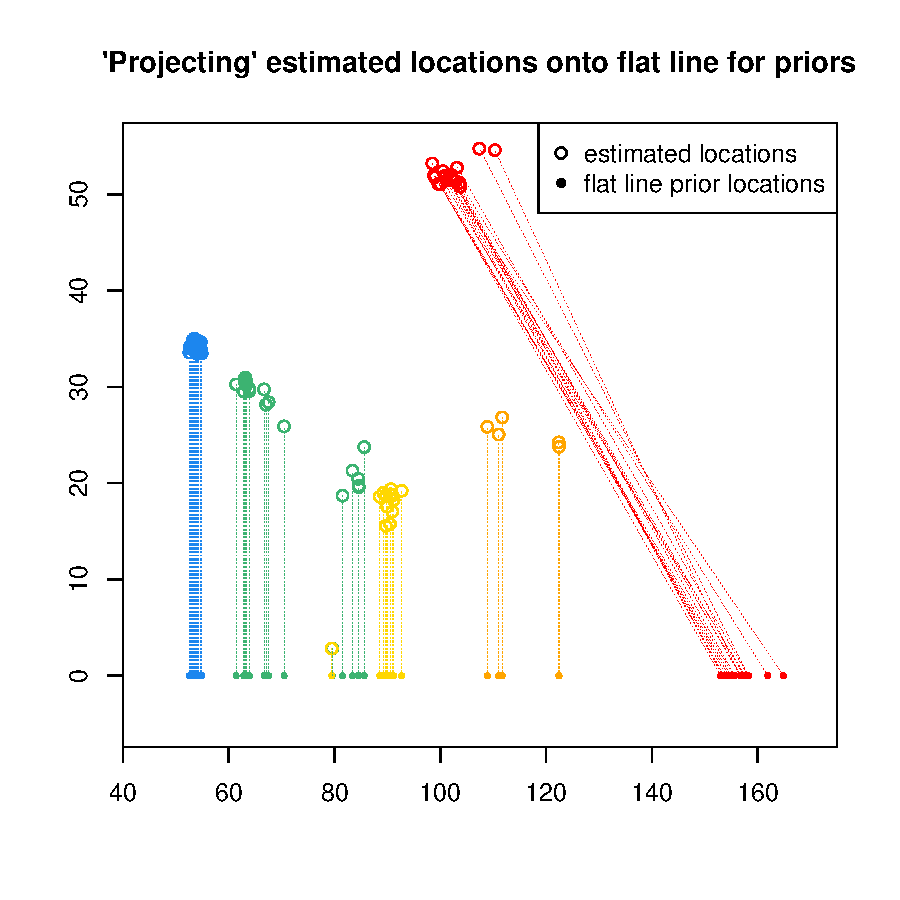
\includegraphics[width=2.8in,height=2.33in]{figs/warblers/warb_inds_on_a_line_setup.pdf}}
		\subcaptionbox{MAP estimate from SpaceMix \label{warb_inds_line_MAP}}
			{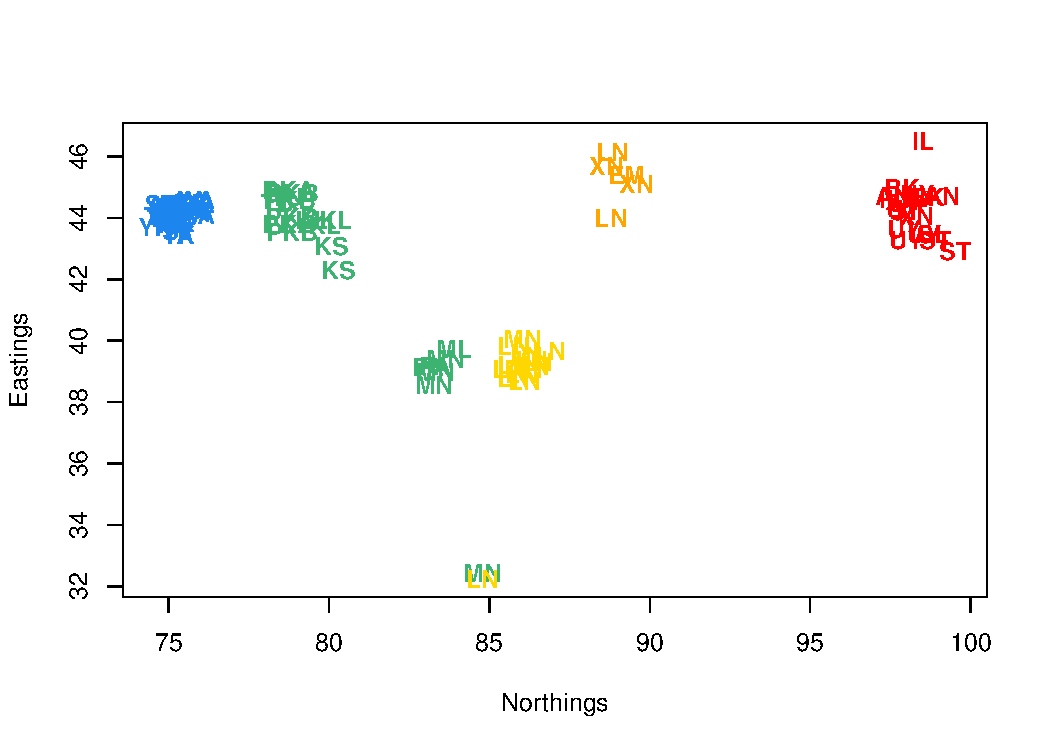
\includegraphics[width=2.8in,height=2.33in]{figs/warblers/warb_inds_on_a_line_MAP1.pdf}}
		\subcaptionbox{Posterior distribution of locations from SpaceMix \label{warb_inds_line_post}}
			{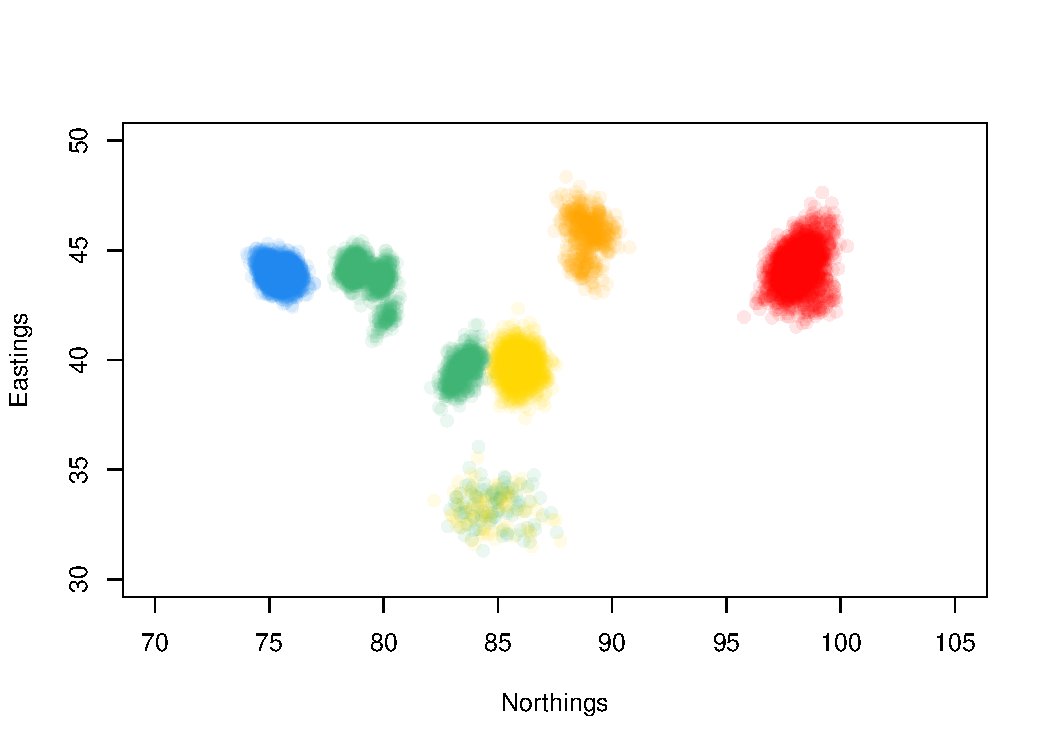
\includegraphics[width=2.8in,height=2.33in]{figs/warblers/warb_inds_on_a_line_post1.pdf}}
	\caption{SpaceMix analyses performed on a warbler individuals for which prior locations are projected onto a flat line in an order that approximately corresponds to their order around the ring: a) the setup of the analysis, in which warbler individuals are projected from their estimated locations in a previous SpaceMix run onto a flat line; b) the MAP estimate of individual locations from a SpaceMix analysis with no admixture, using the flat line locations from (a) as priors on $G^{\prime}$; c) posterior distribution of individual locations from the same analysis.  As with the other inferred maps, here, for clarity, the inferred locations have been rotated via a Procrustes superimposition around their true sampling coordinates.}
	\label{sfig:warb_inds_on_a_line}
\end{figure}


% \paragraph{Speedups}
% Finally, in the interest of computational efficiency, we have implemented several important speed-ups to the calculation of the Wishart likelihood.  The full Wishart probability of the sample standardized covariance matrix, $\widehat{\Omega^{\prime}}$, given the projected parametric covariance matrix, $\identifyadmixsource{\Omega}$, is given below:
% \begin{equation}
% \mathcal{P}(\widehat{\Omega^{\prime}}(X) \; | \; \identifyadmixsource{\Omega}) = \frac{|\widehat{\Omega^{\prime}}|^{ \frac{L - K - 1}{2} } \text{exp} \left(  \frac{-\text{tr}(\frac{\identifyadmixsource{\Omega}^{-1}}{L}\widehat{\Omega^{\prime}})}{2}	\right) }	
% 									{2^{\frac{LK}{2}}  |\frac{\identifyadmixsource{\Omega}}{L}|^{\frac{L}{2}}  \Gamma_{p}\!\left(  \frac{L}{2} \right)	},
% \label{eq:full_wishart_lnl}
% \end{equation}

% where $\text{tr}$ denotes the trace function, $\Gamma_{p}$ denotes the multivariate gamma function, $L$ the number of independent loci over which the covariance is taken, and $K$ the number of samples.  However, because we are using a Markov chain Monte Carlo approach to parameter inference, we may skip the calculation of any parts of this equation that are constant across parameter values (i.e., they do not depend on $\identifyadmixsource{\Omega}$), as these quantities will cancel out during the calculation of the Metropolis-Hastings acceptance ratio (equation \eqref{eq:MH_algorithm}).  We therefore need only calculate the Wishart likelihood as follows:

% \begin{equation}
% \mathcal{P}(\widehat{\Omega^{\prime}}(X) \; | \; \identifyadmixsource{\Omega}) = \frac{ \text{exp} \left(  \frac{-\text{tr}(\frac{\identifyadmixsource{\Omega}^{-1}}{L}\widehat{\Omega^{\prime}})}{2}	\right) }	
% 									{  |\frac{\identifyadmixsource{\Omega}}{L}|^{\frac{L}{2}}  }.
% \label{eq:simple_wishart}
% \end{equation}

% We calculate the log likelihood of the standardized sample covariance given the parametric covariance matrix, so we express the log of this simplified likelihood as 

% \begin{equation}
% \text{log}\left(	\mathcal{P}(\widehat{\Omega^{\prime}}(X) \; |
% 			 \; \identifyadmixsource{\Omega}) \right) = 
% 			\frac{-1}{2} \text{tr}(\identifyadmixsource{\Omega}^{-1}\widehat{\Omega^{\prime}}) - 
% 									\frac{L}{2} \text{log}\left(  \left|\frac{\identifyadmixsource{\Omega}}{L}\right| \right)\text{.}
% \label{eq:log_simple_wishart}
% \end{equation}

% %%%%%%%%% %%%%%%%%% 


%\section*{Future Directions}

%As noted in the third caveat above, the ancestral populations that have donated to the genetic makeup of modern day samples will not be among the samples in the current analysis, and therefore the inferred geography of admixture may only coarsely approximate the truth (depending on the complexity of the demographic history and the extent to which daughter populations of that ancestral admixture source both resemble their parents and have stayed put, geographically).  The inclusion of ancient DNA samples in the analyzed sample offers an intriguing way forward in getting better representation of the ancestral populations from which the ancestors of modern samples received their admixture.  However, it is also possible to model genetic drift as a spatiotemporal Gaussian process, in which covariance in allele frequencies decays with distance both in space and in time.  In this model, which we are currently developing, ancient DNA samples can `calibrate' allele frequency landscapes at points in the past, and modern day samples may draw admixture from estimated coordinates in space-time.

%Three factors in particular stand out as potential sources of difficulty for the model.  %The first is that there may be empirical datasets for which the assumption of isolation by distance is inappropriate.  

%In taxa that migrate from their sampled locations and breed more or less panmictically elsewhere,
%or for some broadcast spawners, 
%a geogenetic map inferred by SpaceMix may bear no relation to the observed sample locations, and thus may be difficult to parse.  However, cases in which there is little or no concordance between the observed and inferred geography may also prove the most interesting and informative.

%Populations generally cluster with other populations sampled on their continent, and the relative placement of populations is similar to that of their observed geography.  Sub-Saharan African populations are distributed in a manner consistent with their sampled latitude, with the San populations in the South and the Ethiopian populations closest to the Eurasian populations in the North.  North African populations, such as the Moroccan, Tunisian, and Egyptian populations, cluster with Middle Eastern populations such as the Yemeni and the UAE, and are quite close to both the Ethiopian populations and the western European populations, such as the Sicilians, the Cypriots, the Tuscans, and the Sardinians.

%Isolation by distance is, in many ways, a more reasonable null hypothesis of population relatedness than a population phylogeny;  \gb{too compare-y?  should I ditch this?} population structure will only rarely be truly tree-like, and a strictly bifurcating graph is unable to accommodate many geographic scenarios, such as multiple equidistant populations in migration-drift equilibrium.
%We recover evidence for several major population expansions and colonization routes in human pre-history.  
%\plrm{``observed pairwise'' should be ``geographic'', here and elsewhere?}



%We can see evidence of these expansions by examining the relationship between observed and estimated pairwise distance between the daughter populations of a putative expansion event.   As can be seen in Figure \ref{sfig:expansion_scenarios}\subref{expansion_inference}, populations that have recently expanded on the landscape are less differentiated both from each other and from their parent population than would be expected from their geographic separation, and this fact is reflected in the decreased ratio between estimated and observed pairwise distances between members of an expansion event.


%\plr{Here the discussion sounds like by default, we'd expect these very different discrete groups, so that placement between them is recent admixture.  That would be true if most modern populations came from one of a few recent expansions.  A different prior would be that populations be uniformly distrubted, making the intermediate popluations expected, and the clustering something to explain.}
%We also see intriguing evidence for potential admixture in the placement of the Chuvash, Uzbekistani, Hazara, and Uygur populations, which choose locations intermediate between Europe and East Asia.  Notably, the Xibo who are sampled from a geographic location close to the Uygur, choose a geogenetic location within the East Asian samples.  The placement of the Moroccan, Mozabite, and Ethiopian populations, which choose locations between the western Eurasian cluster and the African cluster, is also suggestive of potential admixture.  


%%%%%%%%%
%Now instead of occupying an intermediate position the two Ethiopian samples draw a substantial proportion of their ancestry ($\sim 40\%$) from close to where the Egyptian sample has positioned itself in the the middle East cluster. The Sandawe population also draw a substantial portion of their ancestry from the middle east cluster.  Where's the Hadza going? Reciprocally, our North African samples (Egyptian, Tunisian, Morocan, Mozabite), having moved to join the middle eastern populations draw ancestry from close to the Ethiopian samples. 

%Hellenthal et al infer 2 admixture events and 3 admixture sources for the San Khomani: 1 event from the Bantu peoples in South Africa, and 1 event from a combination of northern European and southeast Asian populations.  

%, and we demonstrate the utility of this approach with two empirical applications.

%text for pairwise Pi plots!
To investigate the potential reason for this behavior, we calculated average pairwise sequence divergence at the 2,247 polymorphic loci in the dataset between all 95 individuals and plotted it against the pairwise geographic distance between the individuals (see SuppMat Figure NNN).  The pairwise sequence divergence (0.103) at polymorphic loci between Lud-MN3 and Tro-LN11 is significantly lower than that between any other pair of individuals separated by a comparable distance - lower, in fact, than any comparison between individuals that were not co-located, and lower than any pairwise divergence between any pair of individuals save that between the two Turkish \textit{nitidus} samples. 



 in which we estimate the 2-dimensional configuration of populations that, along with a model of the decay of covariance in allele frequencies with distance, best describes their empirical patterns of genetic differentiation
 
\subsection*{Spatial Admixture Statistic}

\subsection*{Modeling Admixture}
where $f_{\ell,i}$ is the allele frequency in population $i$, $f_{\ell,j}$ is the allele frequency in population $j$, and $p$ is the admixture proportion, which varies between 0 and 1 and describes the extent to which populations $i$ and $j$ are contributing to the genetic make-up of population $k$.

 To infer the spatial context of this admixture, we allow each population a point in space, which we refer to as its source of admixture, from which it draws its admixture, and we model both the location of that source and the extent (proportion) of that admixture.  The observed allele frequencies in sampled populations are therefore a weighted average of the model-estimated allele frequencies at the geographic location of the sampled population and those at the coordinates of the source from which the observed population draws admixture.  That is, the observed allele frequencies in population $k$ are modeled as follows:
 \begin{equation}
 f_{k} = pf_{k'} + (1-p)f_{j},
 \end{equation}
 where $f_{k'}$ are the model-estimated allele frequencies across loci at the spatial location of population $k$ and $f_{j}$ are the model-estimated allele frequencies at the spatial location of the source of admixture $j$, from which population $k$ is drawing admixture in proportion $p$.  The admixture proportion $p$ is constrained to vary between 0 and 0.5, such that at least half of a population's genetic make-up must be determined by its geographic location.

 We re-introduce the population-specific variance terms on each diagonal element of this admixed covariance matrix.  The full expression for our admixed covariance function is below.
 \begin{alignat}{3}
 \label{eq:admixed_covariance_2}
 \Omega^{(*)}_{i,j} = (1-p_i)(1-p_j) \Omega_{i\;,\;j\;} \; \times&\\
 (p_i)(1-p_j) \Omega_{i^{(*)},\;j\;} \; \times   \notag&\\
 (p_j)(1-p_i) \Omega_{i\;,\;j^{(*)}} \; \times   \notag&\\
 (p_i)(p_j) \Omega_{i^{(*)},\;j^{(*)}} \; +   \notag&\\
 \delta_{i,j} \bar{S_k}^{-1} + \delta_{i,j} \eta_k \phantom{+} \notag&
 \end{alignat}

 where $I$ is the identity matrix, $\bar{S_k}$ is the mean sample size in population $k$ across all loci, and $\eta_k$ is the nugget estimated in population $k$.

\section*{Inference}
For details on our Bayesian inference framework and Markov chain Monte Carlo inference procedure, please see the Section: How I spent the past year!

\begin{figure}
	\centering
		\subcaptionbox{Basic Lattice \label{basic_lattice}}
			{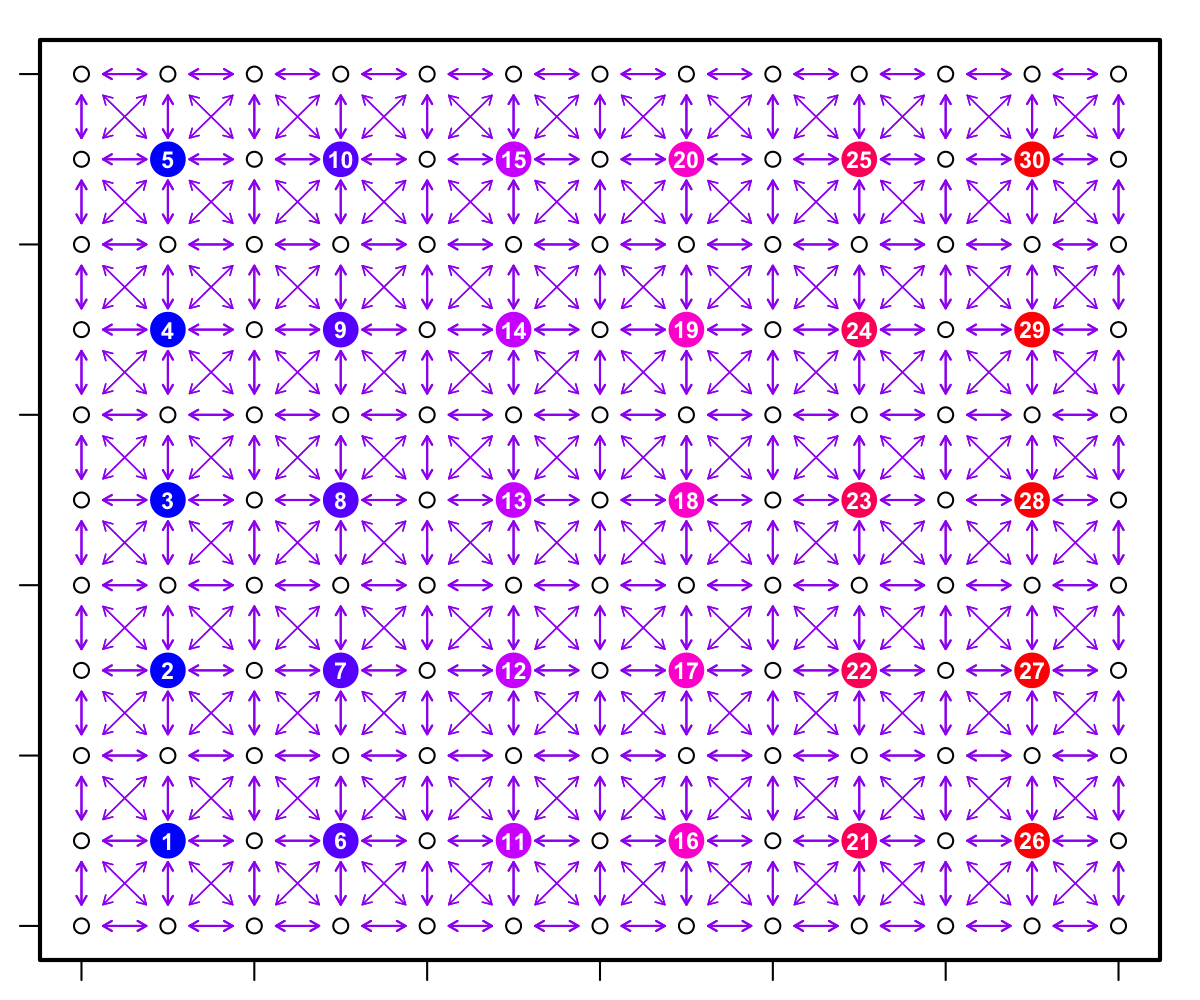
\includegraphics[width=3in,height=2.5in]{figs/sims/basic_lattice.png}}
		\subcaptionbox{Lattice with Barrier \label{barrier_lattice}}
			{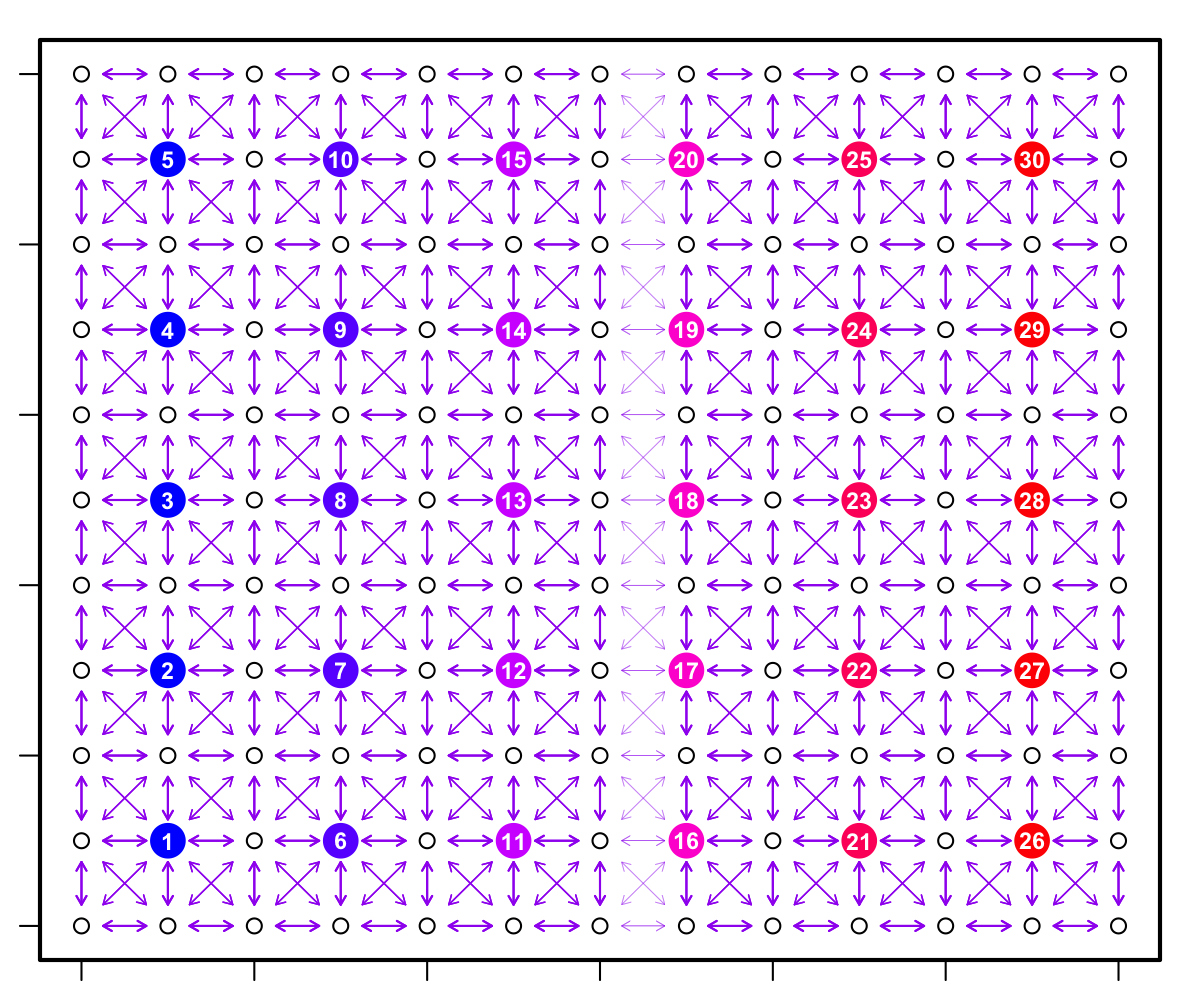
\includegraphics[width=3in,height=2.5in]{figs/sims/barrier_lattice.png}}
		\subcaptionbox{Lattice with Expansion Event \label{barrier_lattice}}
			{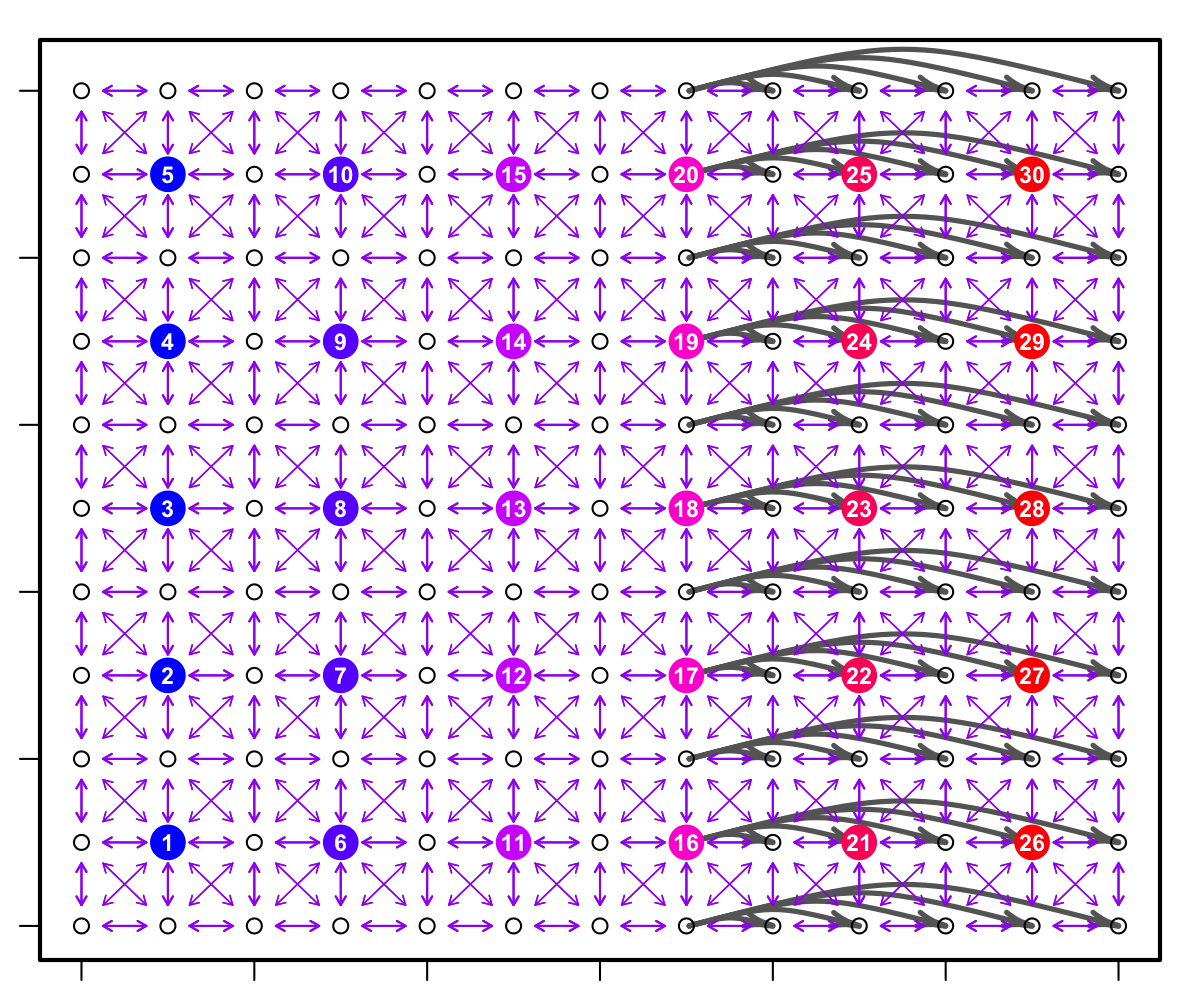
\includegraphics[width=3in,height=2.5in]{figs/sims/expansion_lattice.png}}
	\caption{Different simulation scenarios: (a) basic lattice; (b) lattice with a longitudinal barrier; (c) lattice with expansion event.}\label{sfig:sim_scenarios}
\end{figure}

\begin{figure}[htp!]
	\centering
		{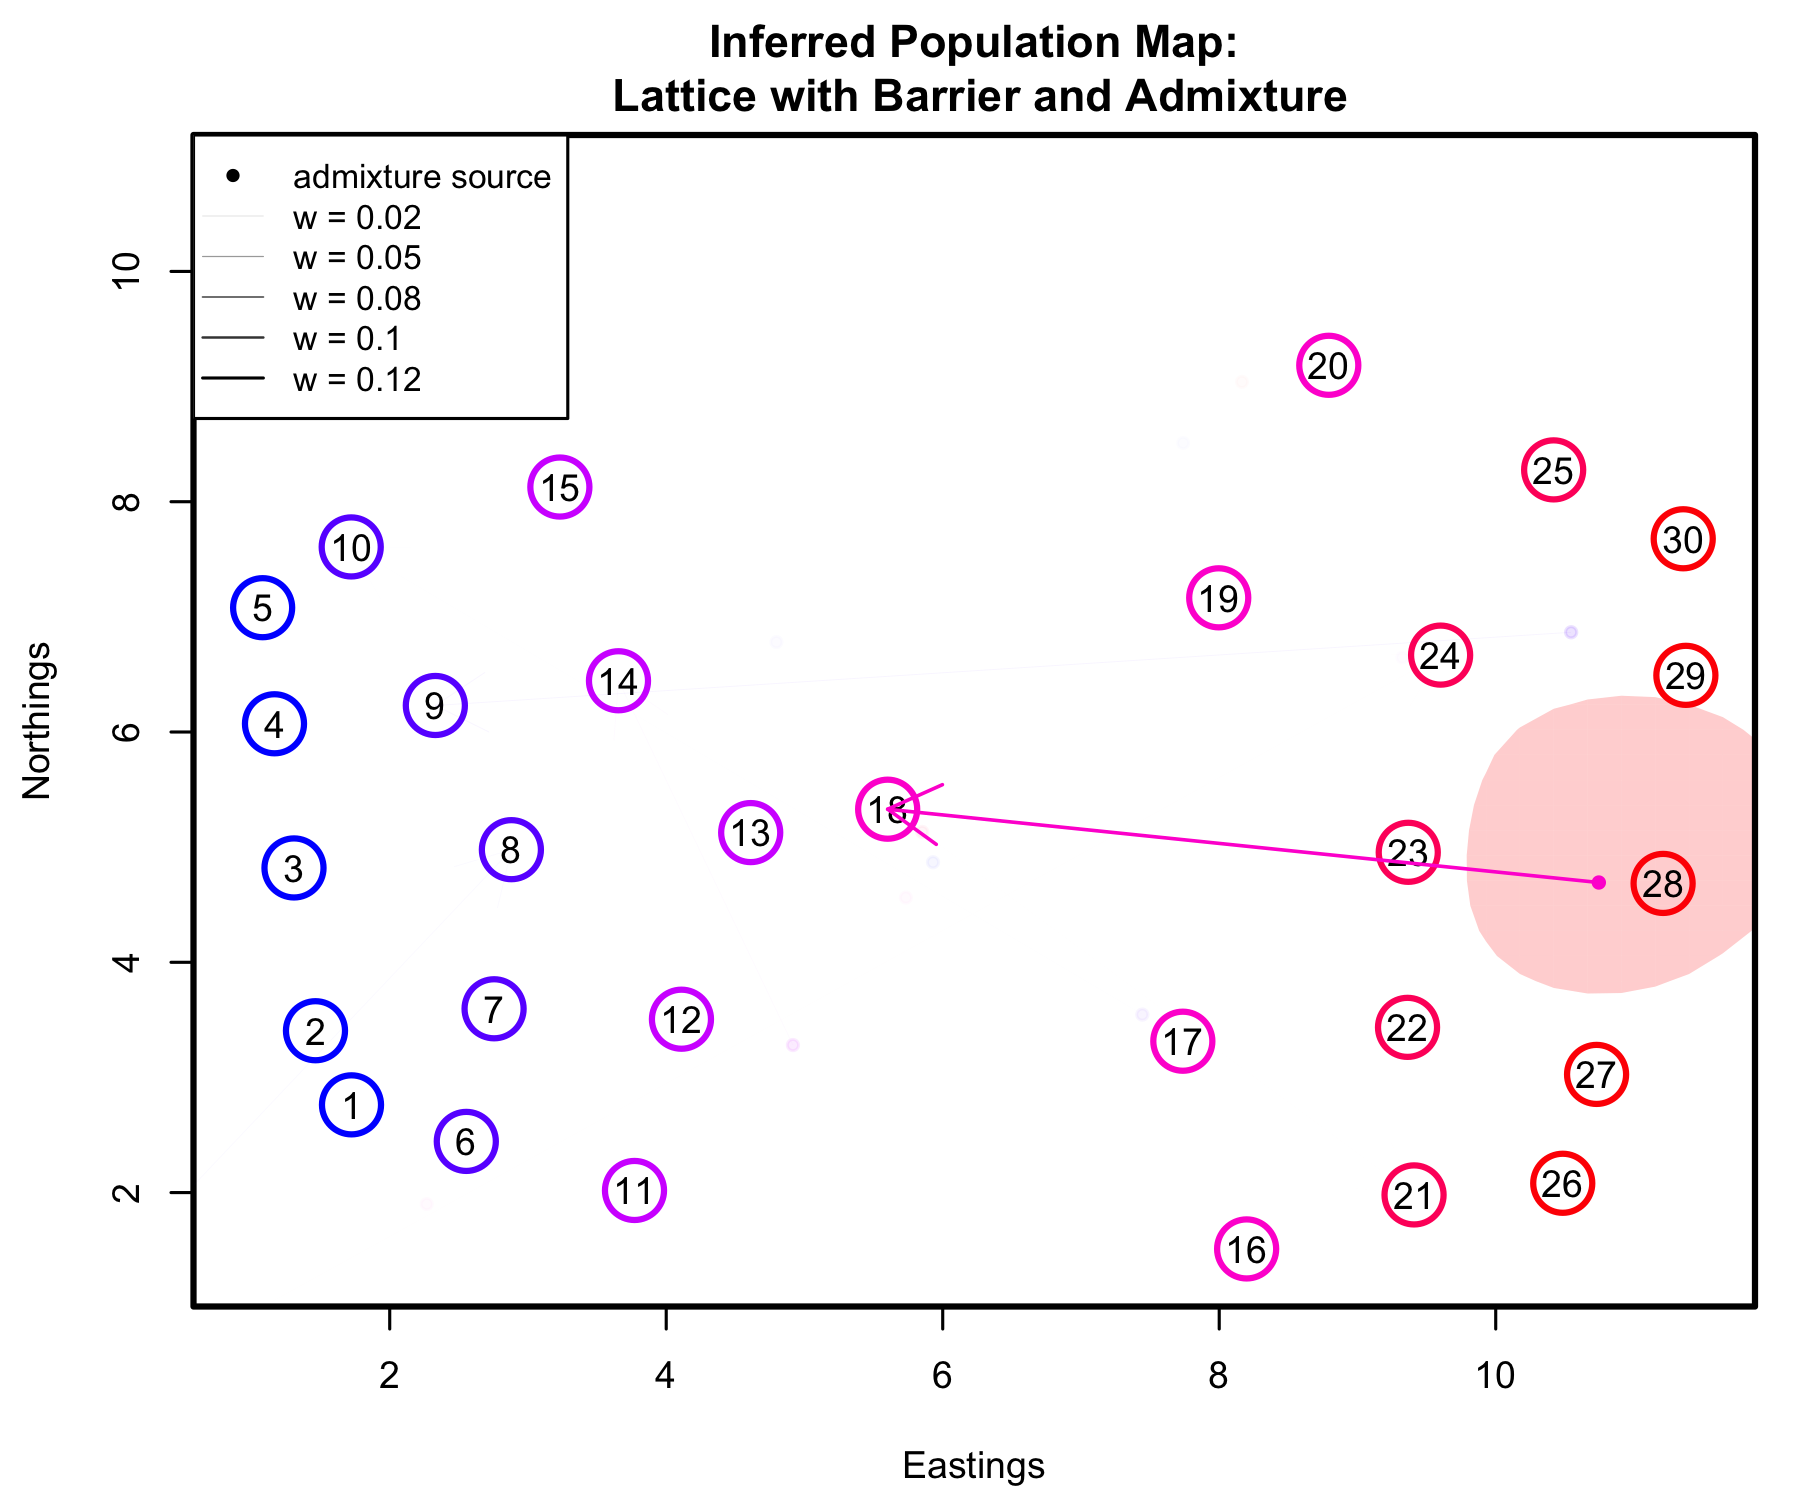
\includegraphics[width=2.4in,height=2in]{figs/sims/GeoGenMap_barr_inland_admixture_2.png}}
	\caption{credible interval of where population 23 draws admixture from.}
\label{sfig:barr_inland_ad_credset}
\end{figure}

\begin{figure}
	\centering
		\subcaptionbox{Lattice \label{lattice_inference}}
			{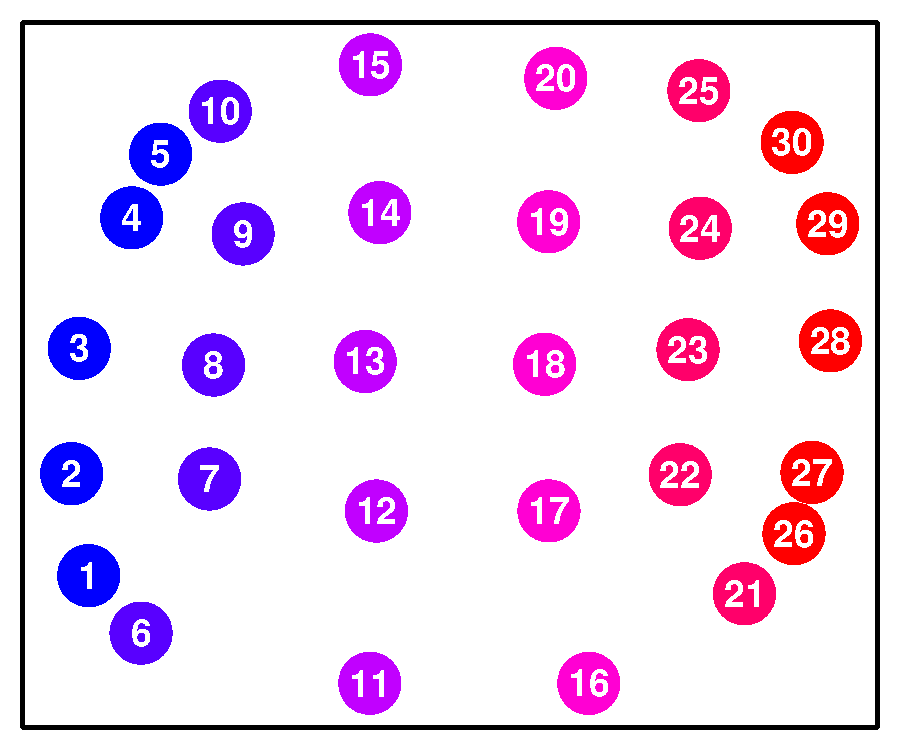
\includegraphics[width=2.8in,height=2.33in]{figs/sims/GeoGenMap_lattice.pdf}}
		\subcaptionbox{Barrier \label{barrier_inference}}
			{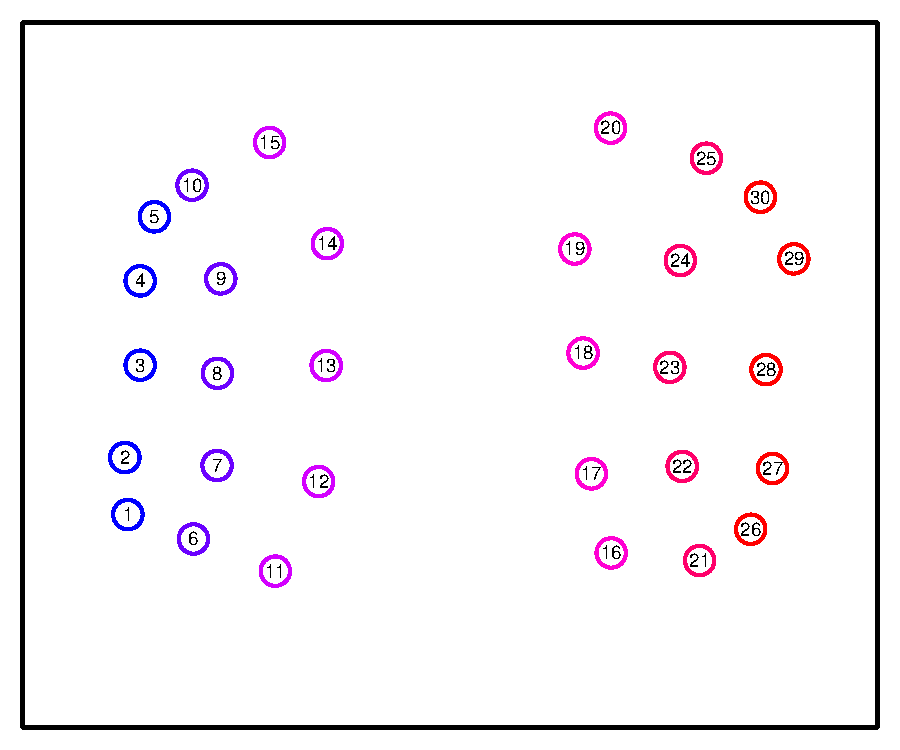
\includegraphics[width=2.8in,height=2.33in]{figs/sims/GeoGenMap_barrier.pdf}}
		\subcaptionbox{Expansion  \label{expansion_inference}}
			{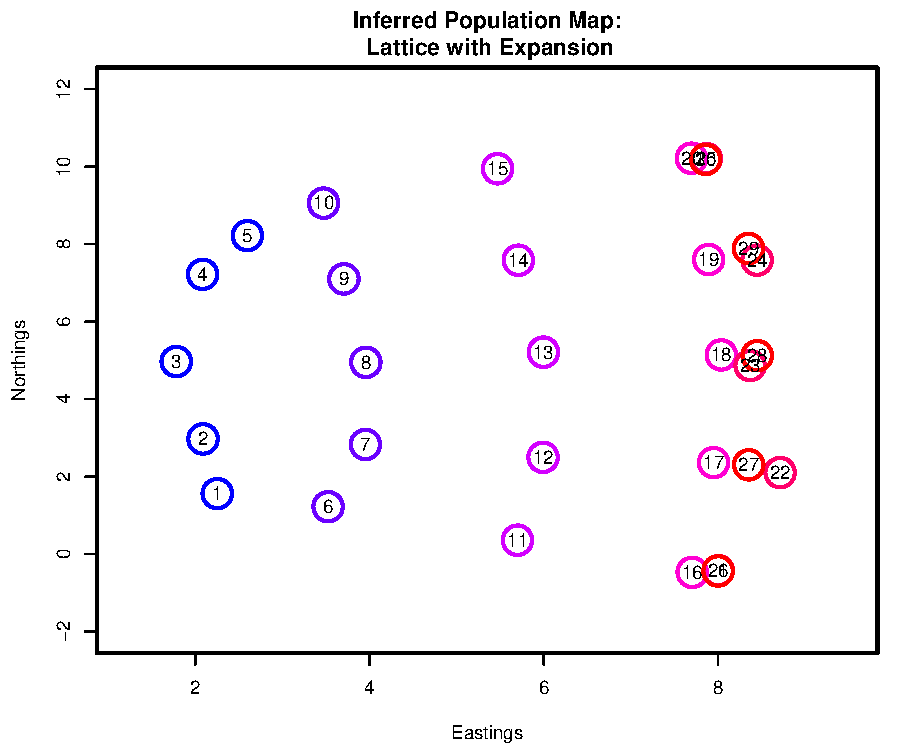
\includegraphics[width=2.8in,height=2.33in]{figs/sims/GeoGenMap_expansion.pdf}}
		\subcaptionbox{Admixture \label{sfig:admixture_inference_CYOL}}
			{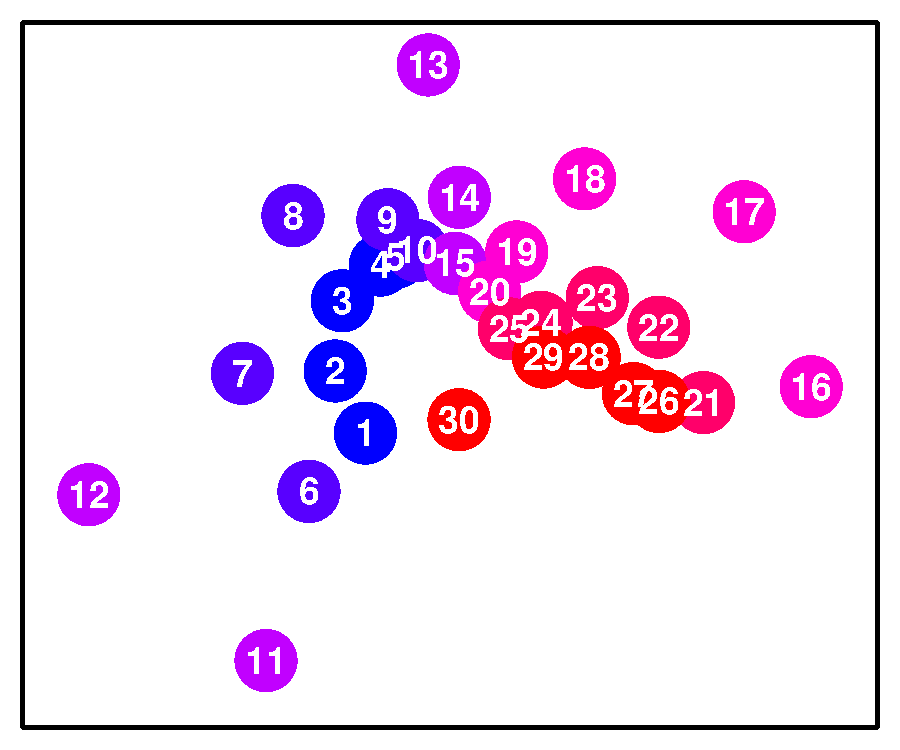
\includegraphics[width=2.8in,height=2.33in]{figs/sims/GeoGenMap_corner_admixture_CYOL.pdf}}
	\caption{Population maps inferred using SpaceMix under three different scenarios: a) simple lattice at equilibrium; b) a lattice with a barrier across the center line of longitude; c) a lattice with recent expansion on the eastern margin; d) a lattice with an admixture event between populations 1 and 30.}\label{sfig:lattice_scenarios}
\end{figure}


\begin{figure}
	\centering
		\subcaptionbox{Location Inference \label{sfig:admixture_inference_CYOL}}
			{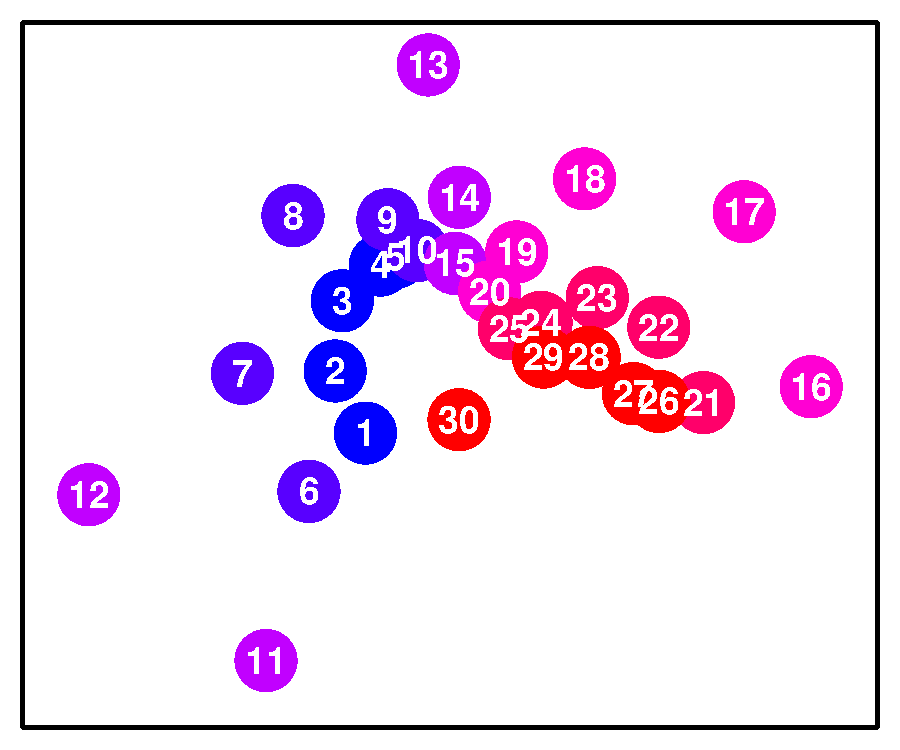
\includegraphics[width=2.4in,height=2in]{figs/sims/GeoGenMap_corner_admixture_CYOL.pdf}}
		\subcaptionbox{Location and Admixture Inference \label{sfig:admixture_inference_CYOL}}
			{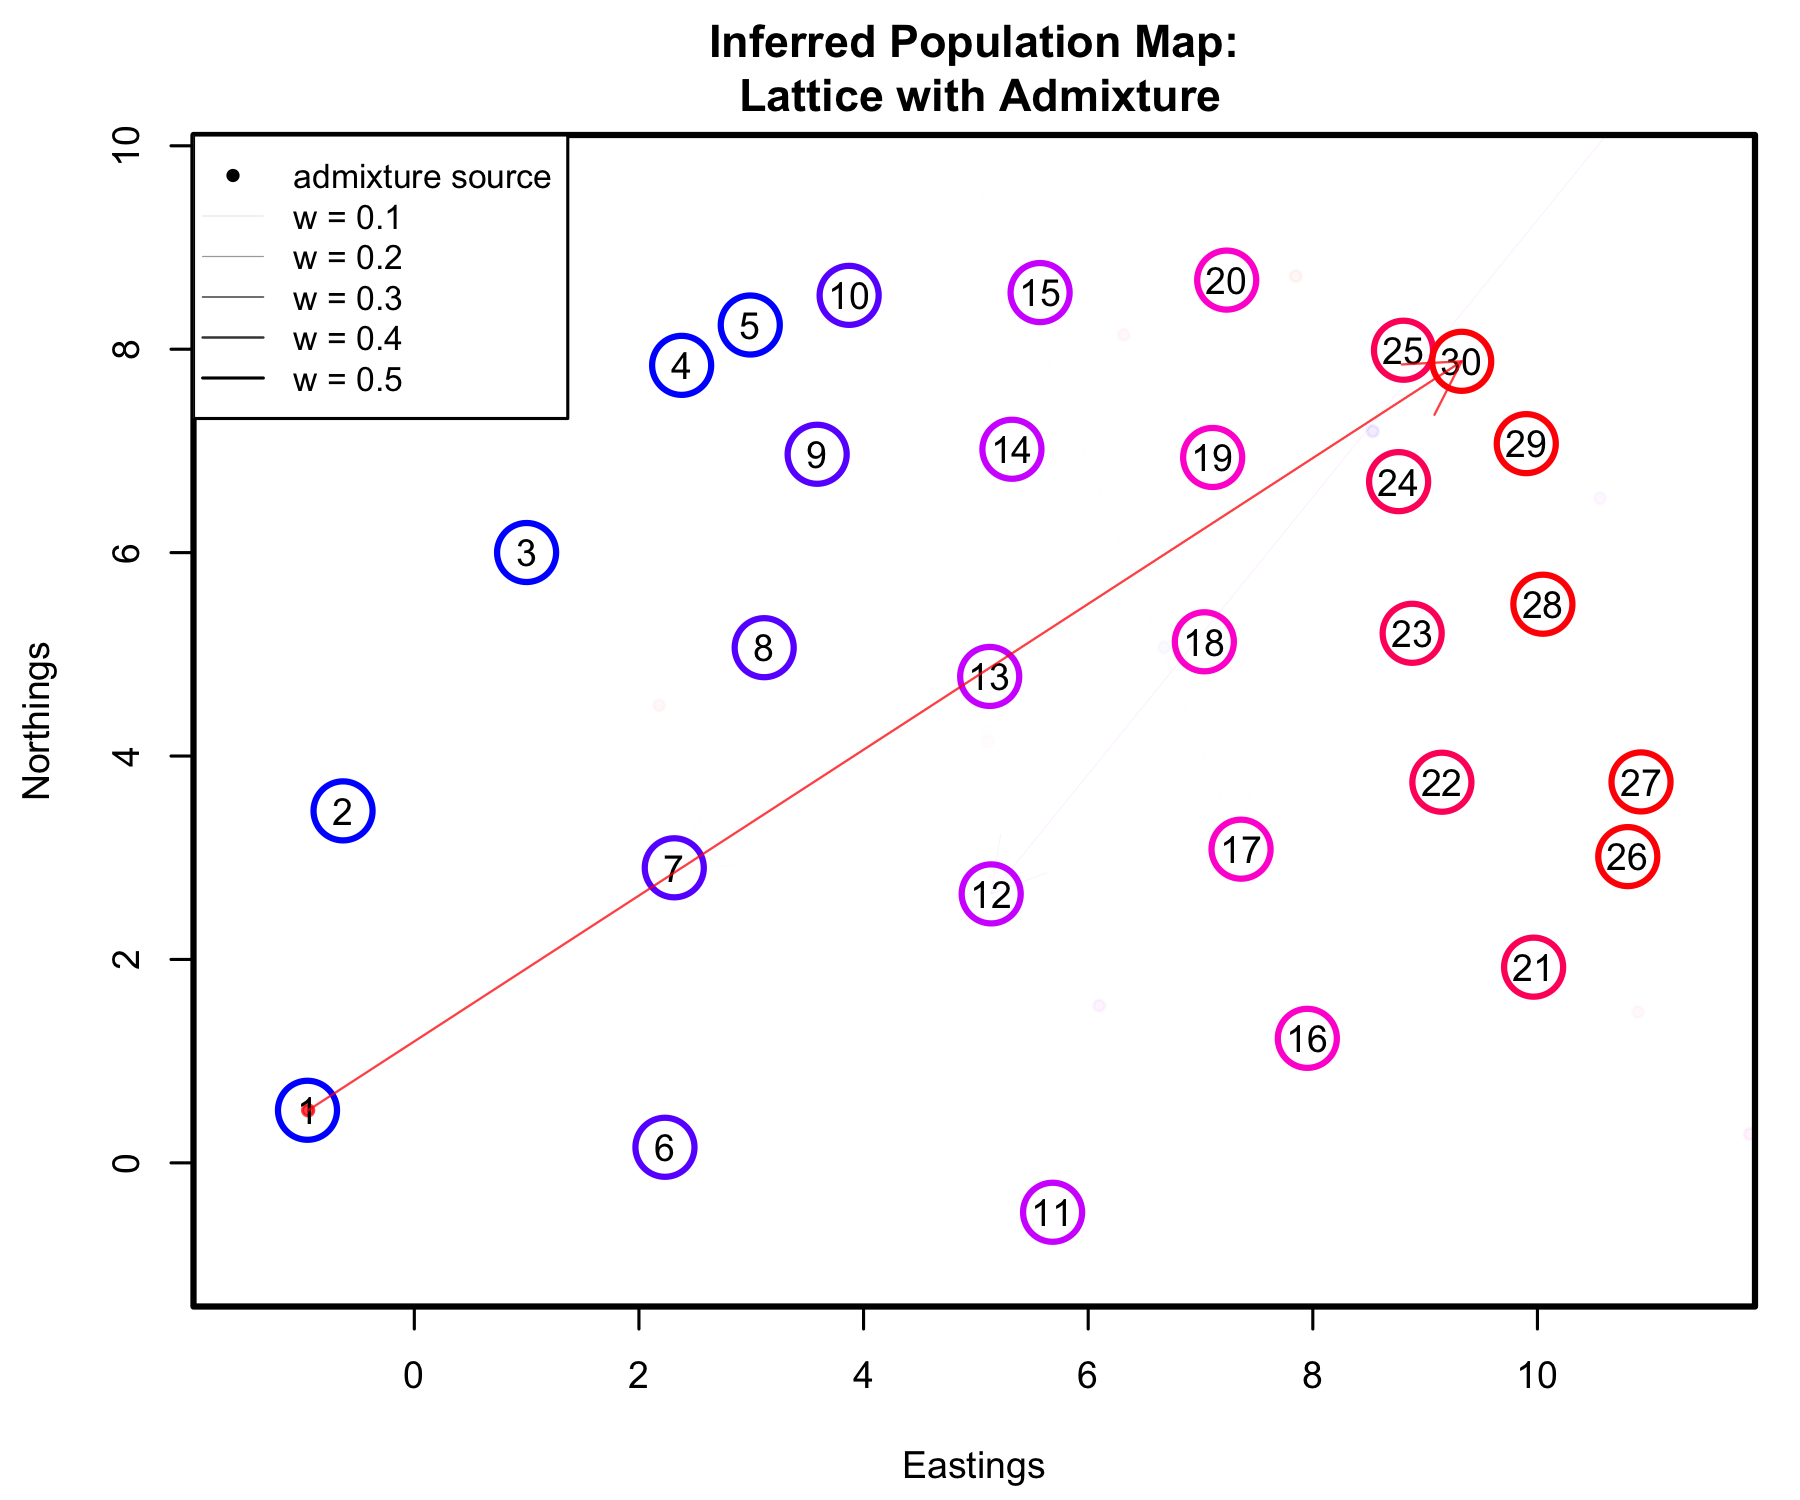
\includegraphics[width=2.4in,height=2in]{figs/sims/GeoGenMap_corner_admixture.png}}
	\caption{Inference of population locations in the scenario depicted in Figure \ref{sfig:admixture_scenario}.  Population 30 has received half of its lineages from population 1, to simulate a long distance admixture event in the very recent past. a) Inference of population locations; b) inference of both population locations and their sources of admixture}\label{sfig:corner_admixture_inference}
\end{figure}

\begin{figure}
	\centering
		\subcaptionbox{Lattice \label{lattice_inference}}
			{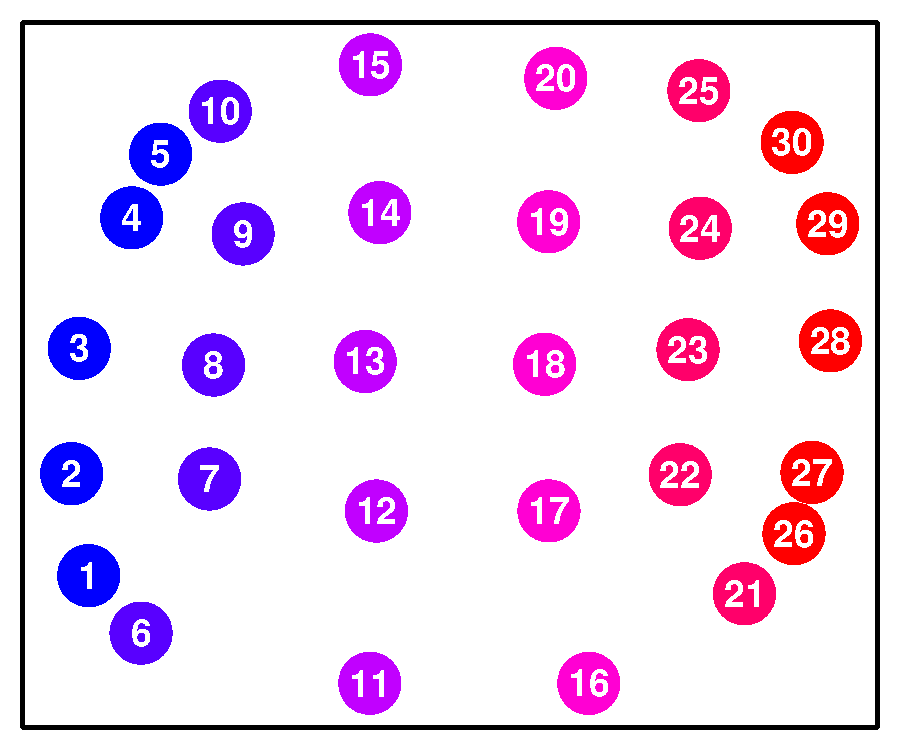
\includegraphics[width=2.8in,height=2.33in]{figs/sims/GeoGenMap_lattice.pdf}}
		\subcaptionbox{Barrier \label{barrier_inference}}
			{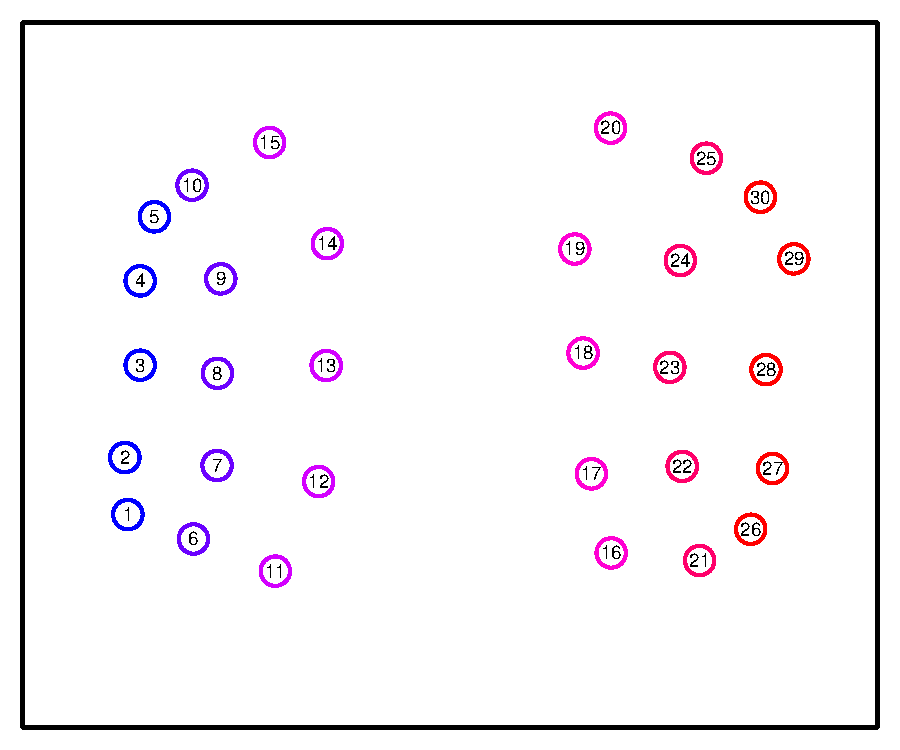
\includegraphics[width=2.8in,height=2.33in]{figs/sims/GeoGenMap_barrier.pdf}}
		\subcaptionbox{Expansion  \label{expansion_inference}}
			{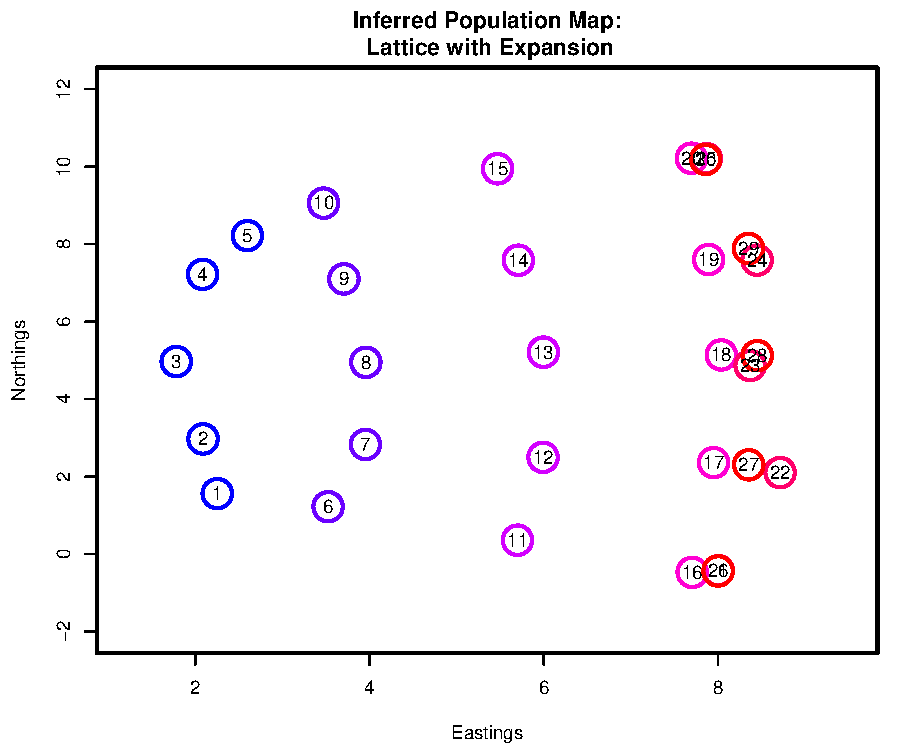
\includegraphics[width=2.8in,height=2.33in]{figs/sims/GeoGenMap_expansion.pdf}}
		\subcaptionbox{Admixture \label{sfig:admixture_inference_CYOL}}
			{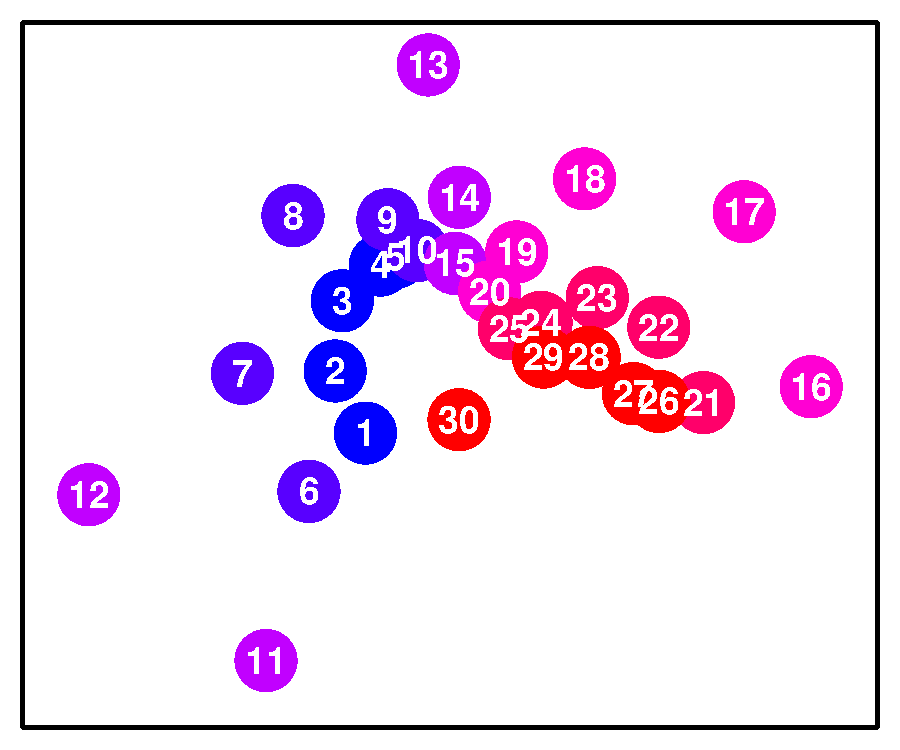
\includegraphics[width=2.8in,height=2.33in]{figs/sims/GeoGenMap_corner_admixture_CYOL.pdf}}
	\caption{Population maps inferred using SpaceMix under three different scenarios: a) simple lattice at equilibrium; b) a lattice with a barrier across the center line of longitude; c) a lattice with recent expansion on the eastern margin; d) a lattice with an admixture event between populations 1 and 30.}\label{sfig:lattice_scenarios}
\end{figure}


\begin{figure}
	\centering
		\subcaptionbox{Location Inference \label{sfig:admixture_inference_CYOL}}
			{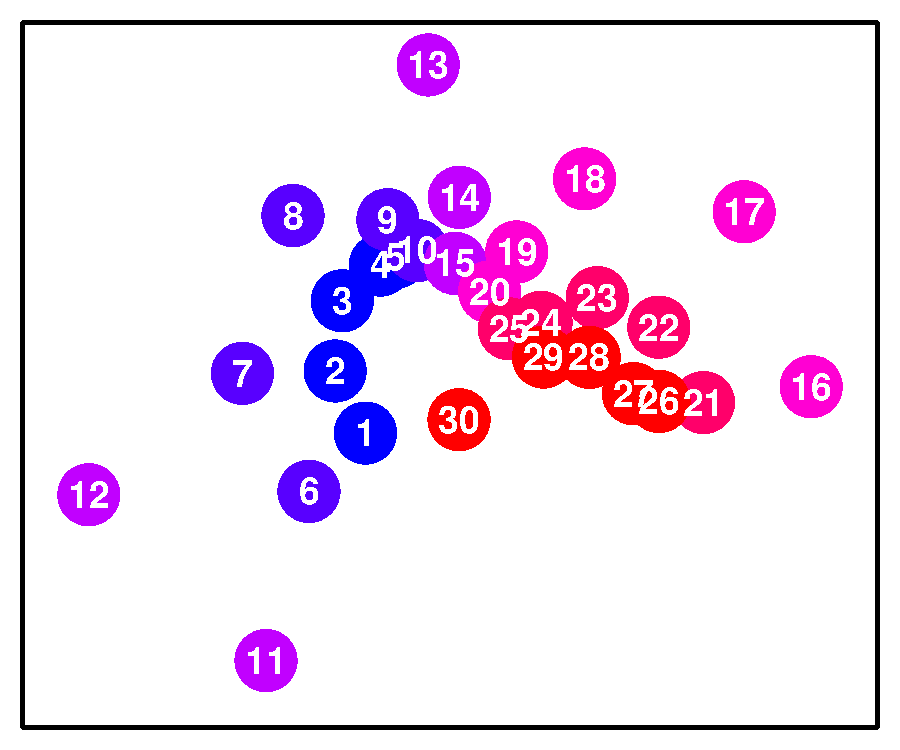
\includegraphics[width=2.4in,height=2in]{figs/sims/GeoGenMap_corner_admixture_CYOL.pdf}}
		\subcaptionbox{Location and Admixture Inference \label{sfig:admixture_inference_CYOL}}
			{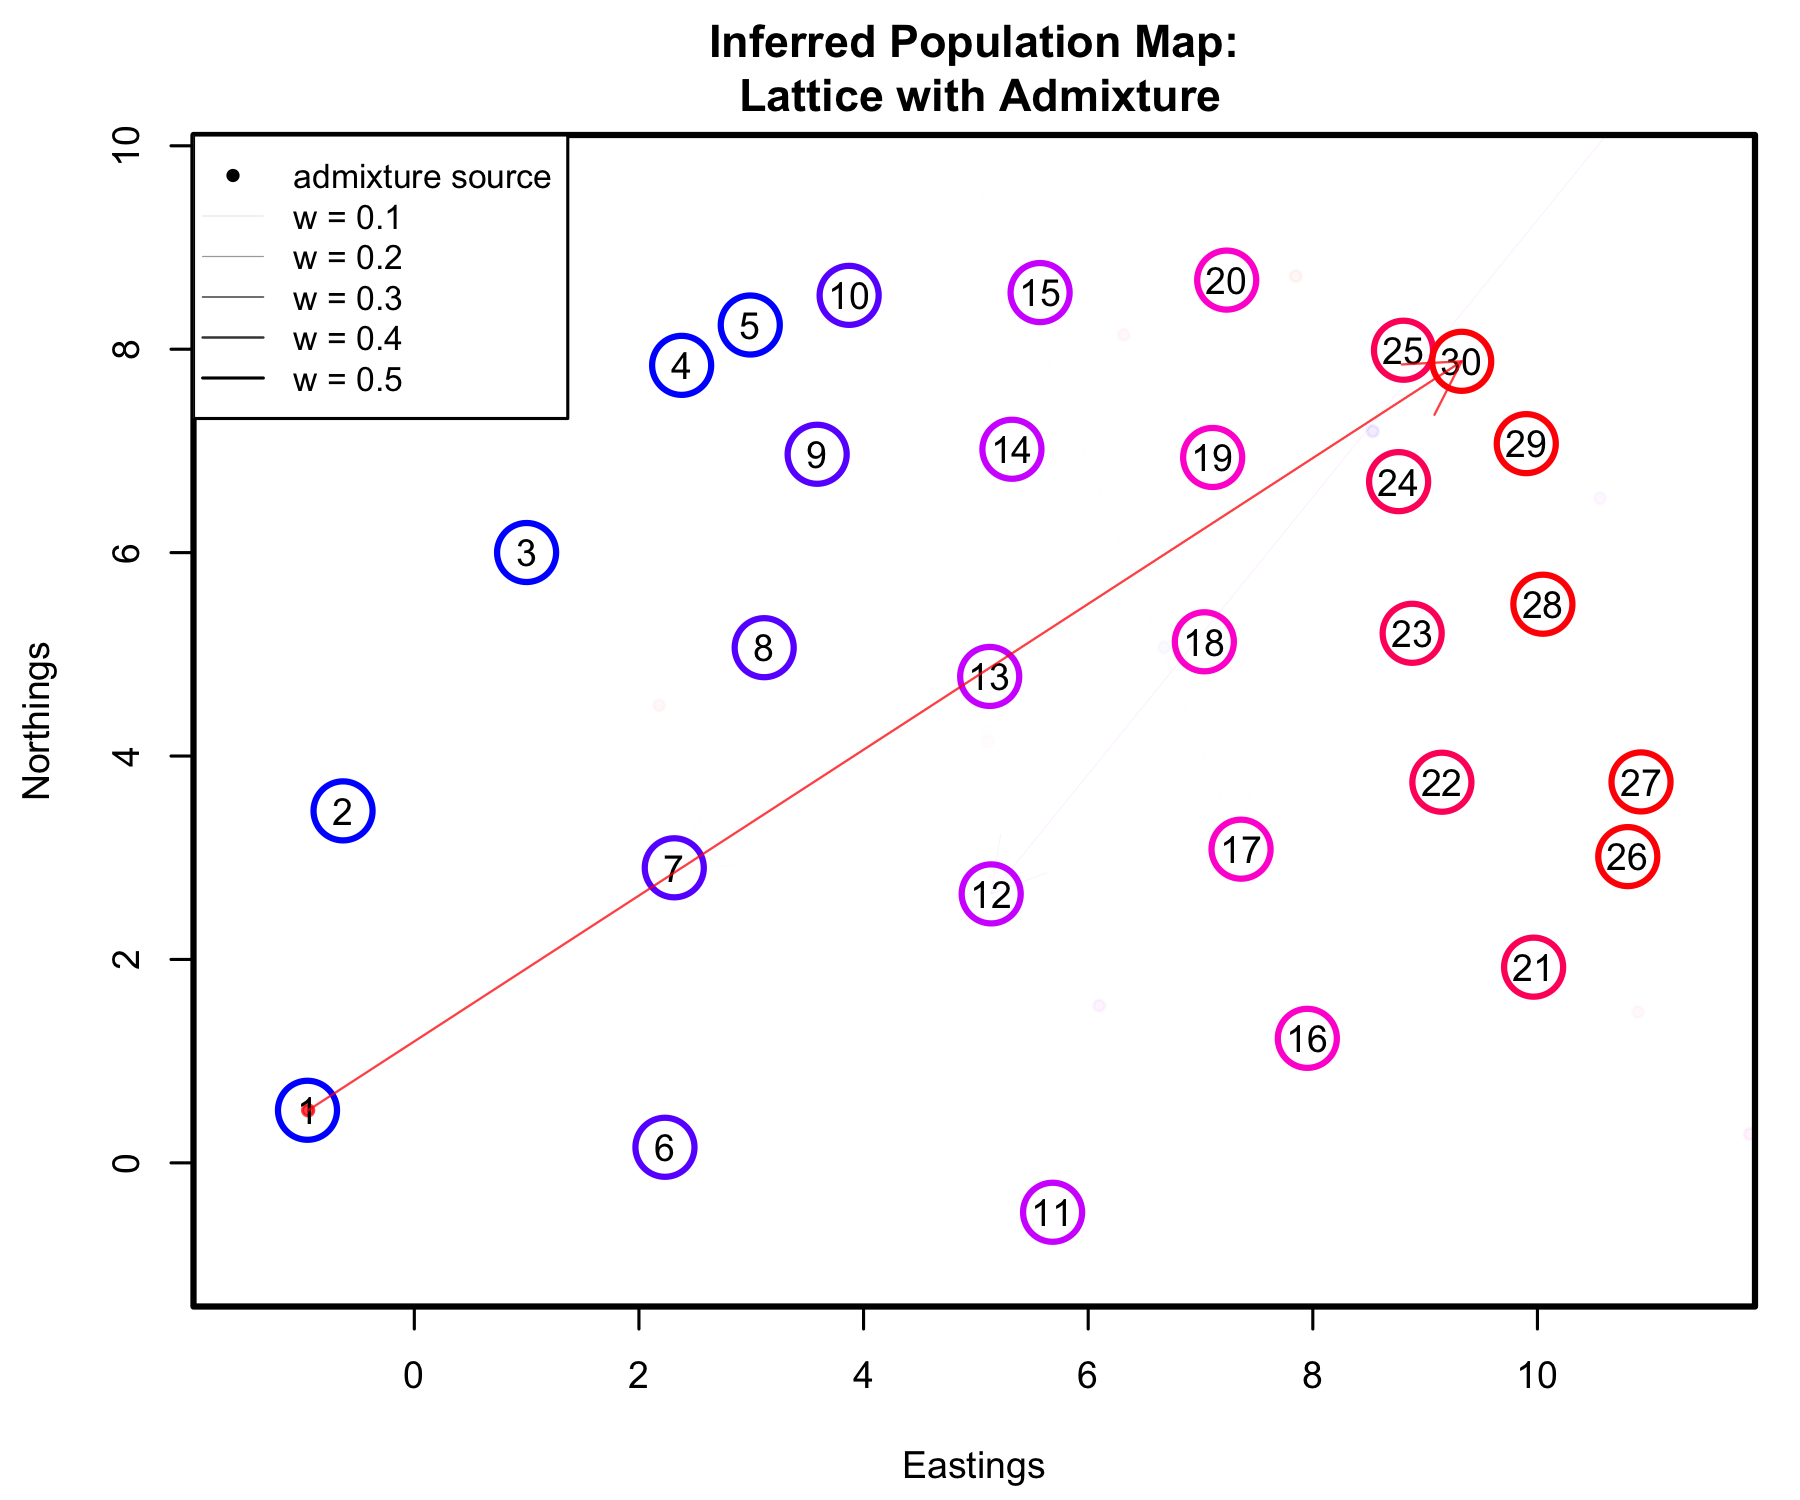
\includegraphics[width=2.4in,height=2in]{figs/sims/GeoGenMap_corner_admixture.png}}
	\caption{Inference of population locations in the scenario depicted in Figure \ref{sfig:admixture_scenario}.  Population 30 has received half of its lineages from population 1, to simulate a long distance admixture event in the very recent past. a) Inference of population locations; b) inference of both population locations and their sources of admixture}\label{sfig:corner_admixture_inference}
\end{figure}

\begin{figure}[htp!]
	\centering
	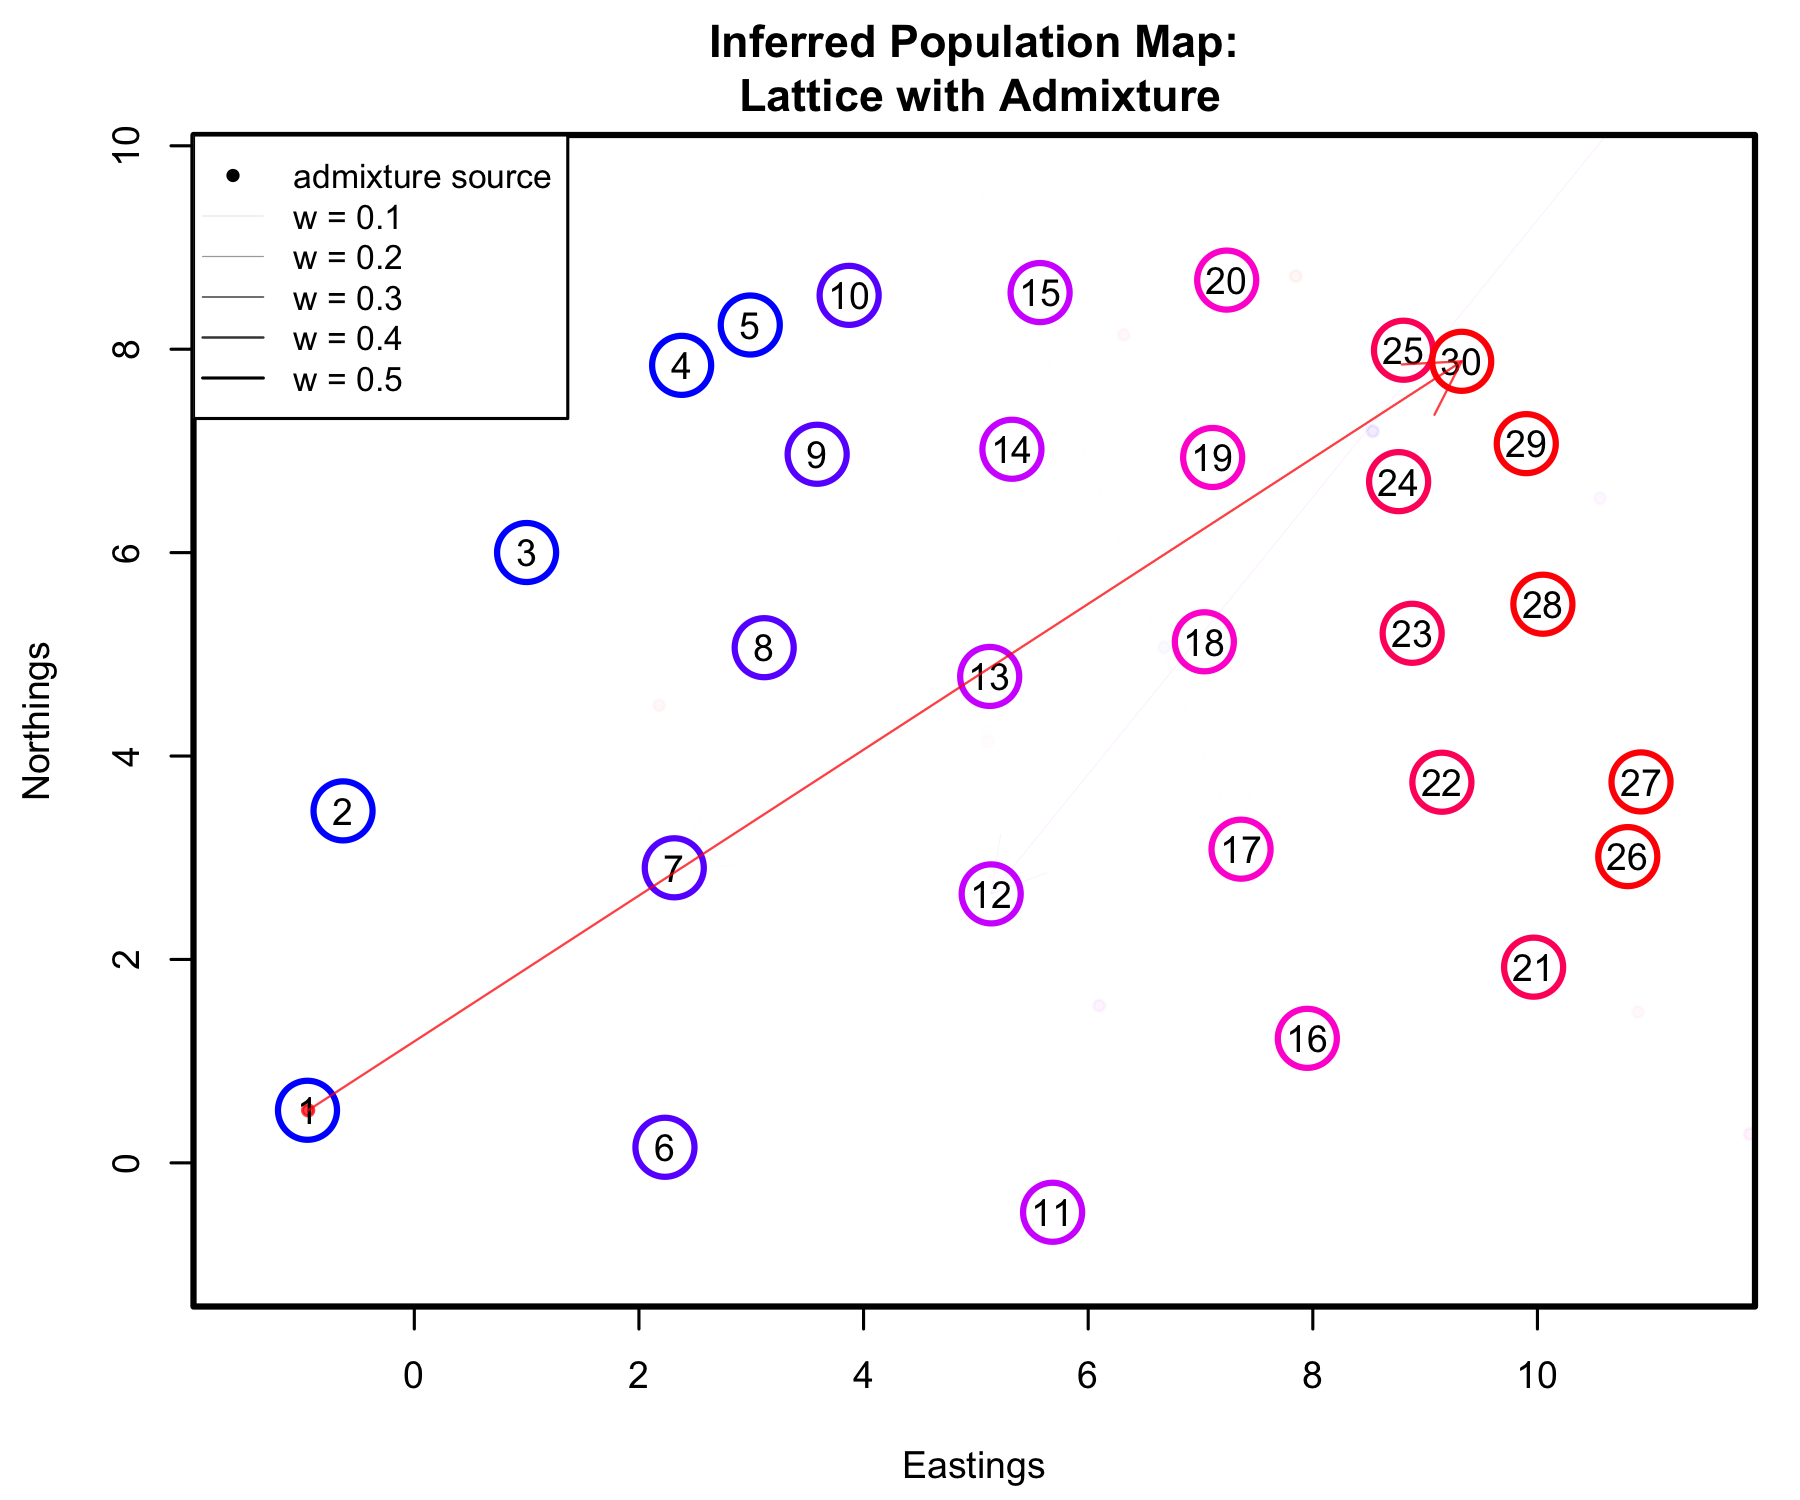
\includegraphics[width=2.4in,height=2in]{figs/sims/GeoGenMap_corner_admixture.png}
	\caption{Posterior distribution of inference of the sources and strengths of admixture for the sampled populations.  The admixed population (Population 30) is drawing admixture from the location of its source of admixture that was used to simulate the data (the location of Population 1).}\label{sfigGeoGenMap_corner_admixture}
\end{figure}


\begin{figure}
	\centering
		\subcaptionbox{Simulated Lattice \label{simple_lattice}}
			{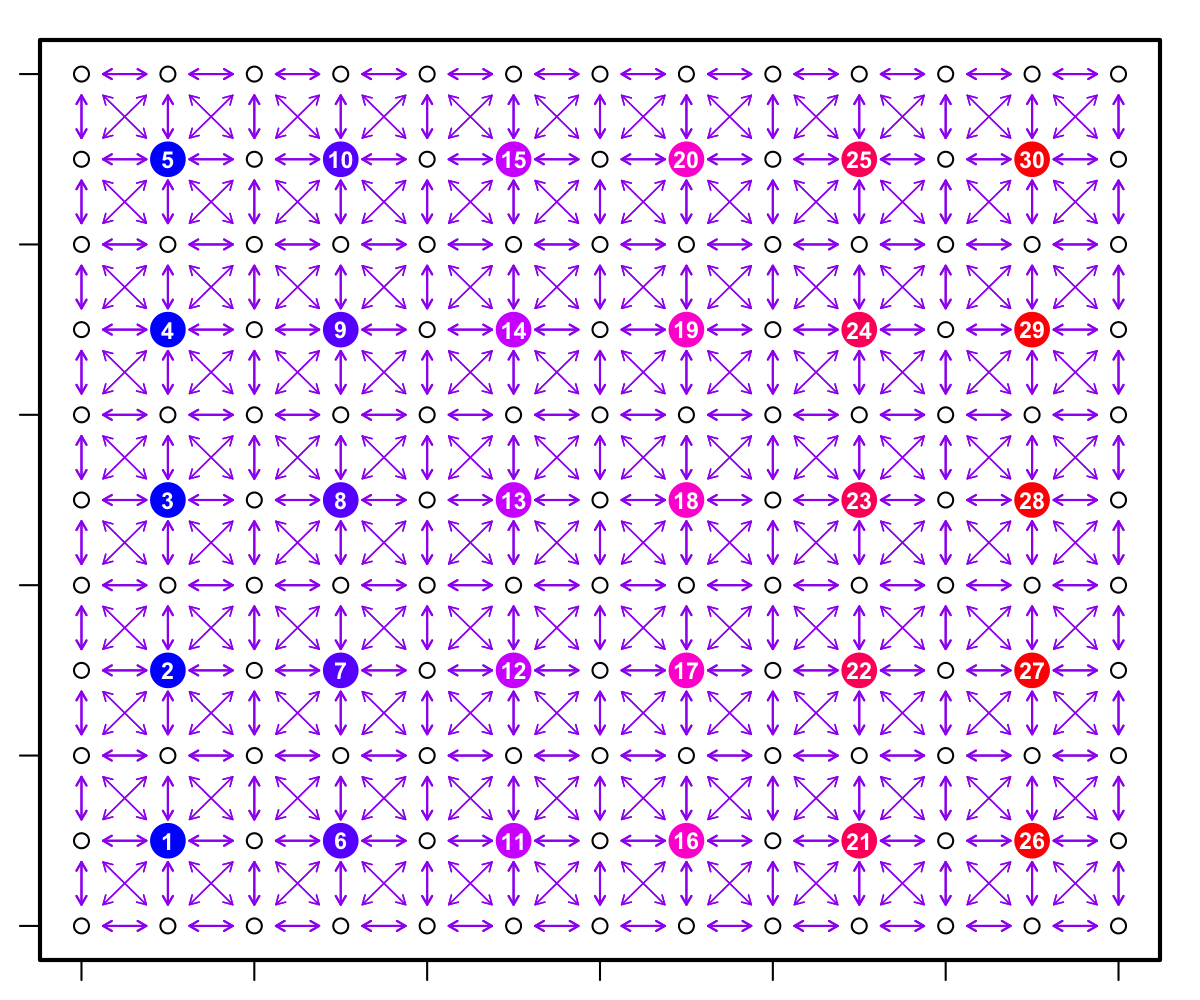
\includegraphics[width=2.8in,height=2.33in]{figs/sims/basic_lattice.png}}
		\subcaptionbox{Lattice \label{lattice_inference}}
			{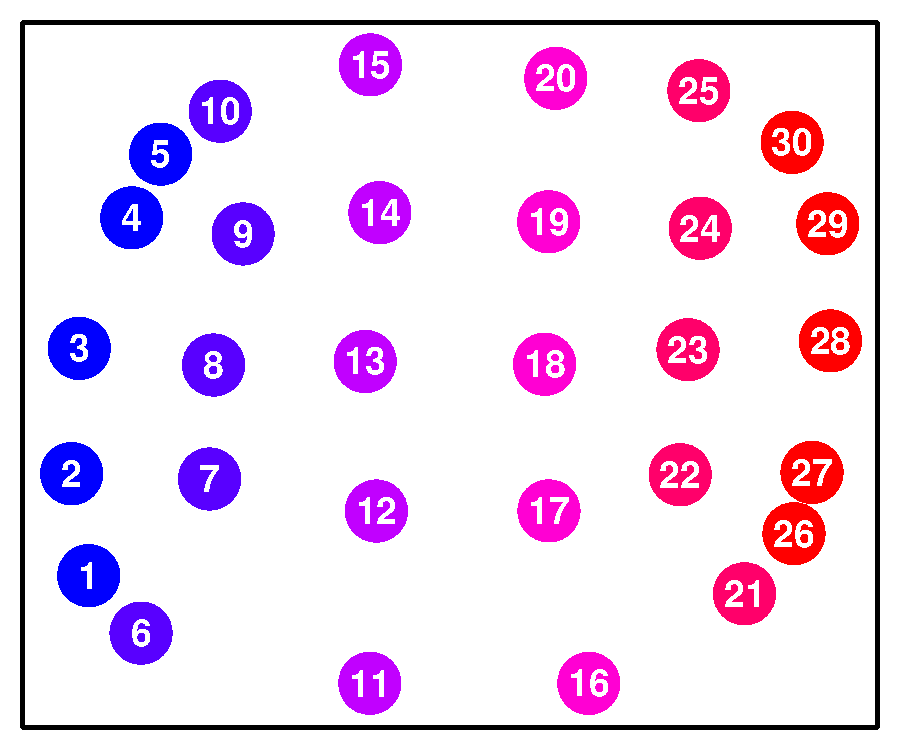
\includegraphics[width=2.8in,height=2.33in]{figs/sims/GeoGenMap_lattice.pdf}}
		\subcaptionbox{Barrier \label{barrier_inference}}
			{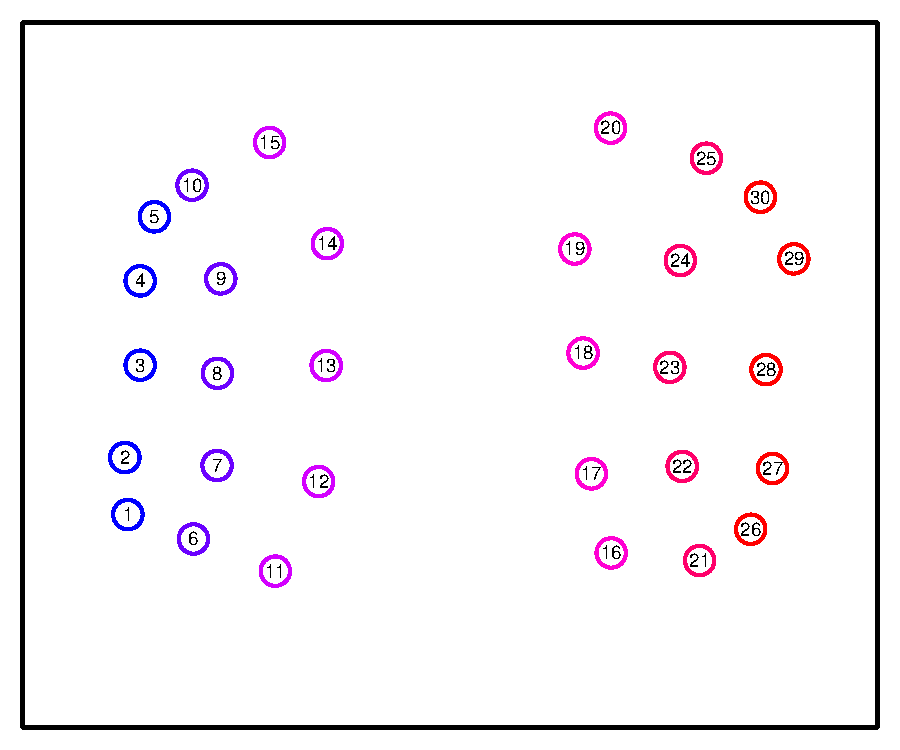
\includegraphics[width=2.8in,height=2.33in]{figs/sims/GeoGenMap_barrier.pdf}}
		\subcaptionbox{Expansion  \label{expansion_inference}}
			{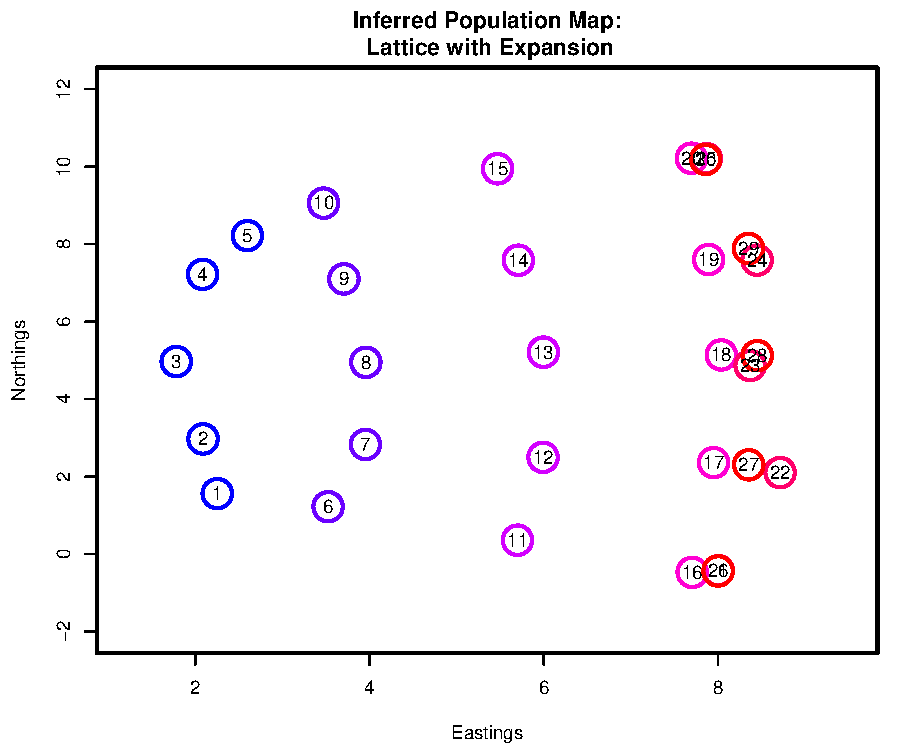
\includegraphics[width=2.8in,height=2.33in]{figs/sims/GeoGenMap_expansion.pdf}}
	\caption{Population maps inferred using SpaceMix under three different scenarios: a) configuration of simulated populations; (c) simple lattice at equilibrium; c) a lattice with a barrier across the center line of longitude; d) a lattice with recent expansion on the eastern margin.}\label{sfig:lattice_scenarios}
\end{figure}
%%%Graham's attempts at arrows in equations
%\begin{equation}
%\source{A}~~~~B~~~~ \target{C}~~~~D
%\drawarrows
%\end{equation}
%blah blah

% \begin{equation}
%   A~~~~B\tikzmark{b} ~~~~ C~~~~\tikzmark{a}D
%   \tikz[overlay,remember picture]
%    {\draw[->,square arrow] (a.south) to (b.south);}
% \end{equation}
% blah blah
% \begin{equation}
%   A~~~~B\tikzmark{b} ~~~~ C~~~~\tikzmark{a}D
%   \tikz[overlay,remember picture]
%    {\draw[->,square arrow] (a.south) to (b.south);}
% \end{equation}
 
 
%\newcommand{\tikzmark}[1]{\tikz[overlay,remember picture] \node (#1) {};}
%\tikzset{square arrow/.style={to path={-- ++(0,-.25) -| (\tikztotarget)}}}

%\begin{equation}
 % a\tikzmark{a}x^2 + bx + c = 5\tikzmark{b}x^2 + bx + c.
 % \tikz[overlay,remember picture]
 %  {\draw[->,square arrow] (a.south) to (b.south);}
%\end{equation}


%%Graham's attempts at arrows in equations 
% \newcommand{\tikzmark}[1]{\tikz[overlay,remember picture] \node (#1) {};}
% \tikzset{square arrow/.style={to path={-- ++(0,-.25) -| (\tikztotarget)}}}


% \newcommand\source[1]{%
%     \tikz[remember picture,baseline,inner sep=0pt] {%
%         \node [name=source,anchor=base]{$#1$};
%     }%
%     \setcounter{target}{0}
% }

% \newcounter{target}
% \newcommand\target[1]{%
%     \tikz[remember picture,baseline,inner sep=0pt] {%
%         \node [name=target-\thetarget,anchor=base]{$#1$};
%     }%
%     \stepcounter{target}%
% }

% \newcommand\drawarrows{
%     \tikz[remember picture, overlay, bend left=20, -latex] {
%         \foreach \i [evaluate=\i as \n using int(\i-1)] in {1,...,\thetarget} {
%             \draw (source.north) to (target-\n.north);
%         }
%     }
% }


% \newcommand\newdrawarrows{
%     \tikz[remember picture, overlay, bend left=20, -latex] {
%         \foreach \i [evaluate=\i as \n using int(\i-1)] in {1,...,\thetarget} {
%             \draw (target-\n.north) to (source.north);
%         }
%     }
% }

% \gc{BLAH}
% Note, by using the sample mean frequency to mean-center our observations, we lose a degree of freedom, and reduce the covariance across loci between populations (sometimes inducing negative covariance between distant populations). We accommodate the extra sampling noise distortion and the reduced rank of the covariance matrix by assuming that our
% %
% \begin{equation}
% X_{\ell} \sim MVN(0, \Omega^{\prime} )
% \end{equation}
% %
% where $\Omega^{\prime}$ is a simple transform of $\Omega$.  Specifically, 
% %
% \begin{equation}
% \Omega^{\prime} = \Psi^{T}   \Omega   \Psi \text{,}
% \label{eq:projected_covariance}
% \end{equation}
% %
% where
%  %
% $\Psi$ is a projection matrix that is used to project our degenerate covariance matrix back into full rank.  This projection matrix is given by
% \begin{equation}
% \Psi = \text{qr.Q}(\text{qr}(\Upsilon))[,1:(k-1)] \text{,}
% \end{equation}
% %
% where $\text{qr}$ is the QR decomposition, $\text{qr.Q}$ returns the original matrix on which the QR decomposition was performed, and
%  $\Upsilon$, a matrix to mean-center the sample allele frequencies, weighting by the mean sample size in each population, is given by 
% \begin{equation}
% T_{ij} = \delta_{ij}  -  \frac{\bar{S}_j}{\sum\limits_{i=1}^{K} \bar{S}_j	} 
% \end{equation}
% %
% \[ \Upsilon = \left( 
% \begin{array}{cccc}
% 1 - \frac{\bar{S}_1}{\sum\limits_{i=1}^{K} \bar{S}_k	} & -\frac{\bar{S}_2}{\sum\limits_{i=1}^{K} \bar{S}_k	} & \ldots & -\frac{\bar{S}_k}{\sum\limits_{i=1}^{K} \bar{S}_k	} \\
% -\frac{\bar{S}_1}{\sum\limits_{i=1}^{K} \bar{S}_k	} & 1 - \frac{\bar{S}_2}{\sum\limits_{i=1}^{K} \bar{S}_k	} & \ldots & -\frac{\bar{S}_k}{\sum\limits_{i=1}^{K} \bar{S}_k	} \\
% \vdots & \vdots & \ddots  & \vdots	\\
% -\frac{\bar{S}_1}{\sum\limits_{i=1}^{K} \bar{S}_k	} & -\frac{\bar{S}_2}{\sum\limits_{i=1}^{K} \bar{S}_k	} & \ldots  & 1 - \frac{\bar{S}_k}{\sum\limits_{i=1}^{K} \bar{S}_k	} 
% \end{array} \right).\]\\
% %



%  $\Upsilon$, a matrix to mean-center the sample allele frequencies, weighting by the mean sample size in each population, is given by 
% %
% \[ \Upsilon = \left( 
% \begin{array}{cccc}
% 1 - \frac{\bar{S}_1}{\sum\limits_{i=1}^{K} \bar{S}_k	} & -\frac{\bar{S}_2}{\sum\limits_{i=1}^{K} \bar{S}_k	} & \ldots & -\frac{\bar{S}_k}{\sum\limits_{i=1}^{K} \bar{S}_k	} \\
% -\frac{\bar{S}_1}{\sum\limits_{i=1}^{K} \bar{S}_k	} & 1 - \frac{\bar{S}_2}{\sum\limits_{i=1}^{K} \bar{S}_k	} & \ldots & -\frac{\bar{S}_k}{\sum\limits_{i=1}^{K} \bar{S}_k	} \\
% \vdots & \vdots & \ddots  & \vdots	\\
% -\frac{\bar{S}_1}{\sum\limits_{i=1}^{K} \bar{S}_k	} & -\frac{\bar{S}_2}{\sum\limits_{i=1}^{K} \bar{S}_k	} & \ldots  & 1 - \frac{\bar{S}_k}{\sum\limits_{i=1}^{K} \bar{S}_k	} 
% \end{array} \right).\]\\
% %
% The standardized sample allele frequency covariance $\Omega^{\prime}$ is then simply given by $XX^{T}$, and the Wishart likelihood of the standardized sample covariance is taken as a function of the projected parametric covariance matrix as follows:
% %
% \begin{equation}
% \label{eq:projected_wishart_dist}
% P(\widehat{\Omega} \mid \Omega) = \mathcal{W}\left(L \widehat{\Omega^{\prime}} \mid  \Psi^{T}   \Omega   \Psi,L \right) \text{.}
% \end{equation}
%
